\apendice{Especificación de diseño}

\section{Introducción}
Este anexo describe en detalle las decisiones técnicas y la arquitectura adoptada durante la construcción de AgroSkopos. El objetivo de esta fase de diseño es transformar los requisitos analizados en especificaciones tangibles de bases de datos, estructuración algorítmica y despliegue de \textit{software}. Se aborda, de forma escalonada, la estructuración de la persistencia de datos (esquema relacional), el diseño procedimental de la lógica algorítmica, y por último, la arquitectura global del sistema mediante diagramas.

\section{Diseño de datos}

\subsection{Arquitectura y justificación de la base de datos}
El diseño arquitectónico de la persistencia de datos persigue como premisa fundamental la \textbf{simplicidad y el pragmatismo}. En lugar de sobredimensionar el esquema con decenas de tablas altamente normalizadas que acabarían fragmentando la telemetría, se ha optado intencionadamente por un modelo de datos conciso y robusto compuesto por seis entidades clave. Esta simplificación estratégica está firmemente justificada por dos motivos fundamentales: en primer lugar, \textbf{maximiza el rendimiento y la velocidad de escritura}, un factor crítico cuando el robot debe enviar ráfagas de telemetría de sensores por segundo; y en segundo lugar, \textbf{reduce la complejidad computacional} en el \textit{backend} a la hora de realizar cruces de información (\textit{JOINs}), facilitando su mantenimiento y lectura.

La capa de persistencia se asienta sobre un sistema gestor de bases de datos relacionales PostgreSQL. La interacción entre el \textit{backend} (Node.js) y la base de datos no se realiza mediante consultas \textbf{SQL} crudas, sino que se gestiona íntegramente a través de un ORM (\textit{Object-Relational Mapping}). La adopción de un ORM abstrae la complejidad de la base de datos, previniendo vulnerabilidades críticas como la inyección \textbf{SQL}, y permite manipular la información utilizando paradigmas orientados a objetos directamente en el código de la aplicación.

Para este proyecto, la elección tecnológica ha recaído sobre \textbf{Prisma ORM}. Frente a alternativas más antiguas como Sequelize o TypeORM, Prisma destaca por autogenerar un cliente de base de datos fuertemente tipado basándose en un único archivo de configuración declarativo (\texttt{schema.prisma}). Esto garantiza que cualquier discrepancia entre el modelo de datos y el código se detecte de forma inmediata en tiempo de compilación (evitando fallos inesperados en producción) y centraliza la gestión de migraciones, simplificando radicalmente la evolución del proyecto y mejorando la experiencia de desarrollo.

\subsection{Entidades del modelo}
El modelo de datos se ha diseñado buscando el equilibrio comentado entre normalización estructural y rendimiento masivo. A continuación, se detallan las entidades principales que componen el sistema:

\begin{itemize}
    \item \textbf{usuarios:} Almacena las credenciales cifradas, el correo electrónico de contacto para notificaciones y los perfiles de acceso (roles, avatares) del personal de la explotación agraria. Mantiene una relación \textit{1 a N} con \textit{misiones} (quién planificó la tarea) y con \textit{ejecuciones\_mision} (quién dio la orden de ejecución).
    \item \textbf{misiones:} Define los parámetros estáticos, espaciales y logísticos de una tarea agronómica. Incluye campos geométricos almacenados en formato JSON (\textit{area\_trabajo}, \textit{puntos\_interes}) así como requisitos operativos (ancho de trabajo, batería mínima requerida). Registra el \textit{usuario\_id} del creador.
    \item \textbf{ejecuciones\_mision:} Actúa como entidad transaccional que registra las métricas temporales de una misión al ser desplegada en el terreno. Controla el estado actual de la ejecución, el progreso, la fecha de inicio/fin y la distancia real recorrida. Mantiene una relación \textit{1 a N} con la tabla \textit{misiones} y asocia opcionalmente el \textit{usuario\_id} del operario que inició la tarea.
    \item \textbf{robot\_datos:} Diseñada para soportar una alta carga de inserciones, esta tabla almacena la telemetría agronómica capturada por los sensores en tiempo real durante una ejecución (niveles de nitrógeno, fósforo, potasio, pH, temperatura del suelo y radiación solar), georreferenciando cada lectura con coordenadas espaciales. Mantiene una relación \textit{1 a N} con \textit{ejecuciones\_mision}.
    \item \textbf{robot\_estado:} Entidad orientada a reflejar el \textit{hardware} en tiempo real. En ella, el robot reporta periódicamente su telemetría de bajo nivel (coordenadas actuales, velocidad, \textit{heading}, temperatura y voltaje de batería).
    \item \textbf{historial\_energia:} Persiste métricas históricas de consumo eléctrico y captación energética del panel solar para permitir el análisis a largo plazo del rendimiento y la autonomía del prototipo.
\end{itemize}

A continuación, en la figura \ref{fig:img/apendice_C/diagrama_bd_final.png}, se expone el Diagrama Entidad-Relación (ER) lógico que ilustra la cardinalidad e interacción semántica entre los dominios principales. Cabe destacar que la estructura visual de este diagrama ha sido autogenerada de manera automática a partir del esquema de configuración de Prisma ORM.

\begin{figure}[!h]
    \centering
    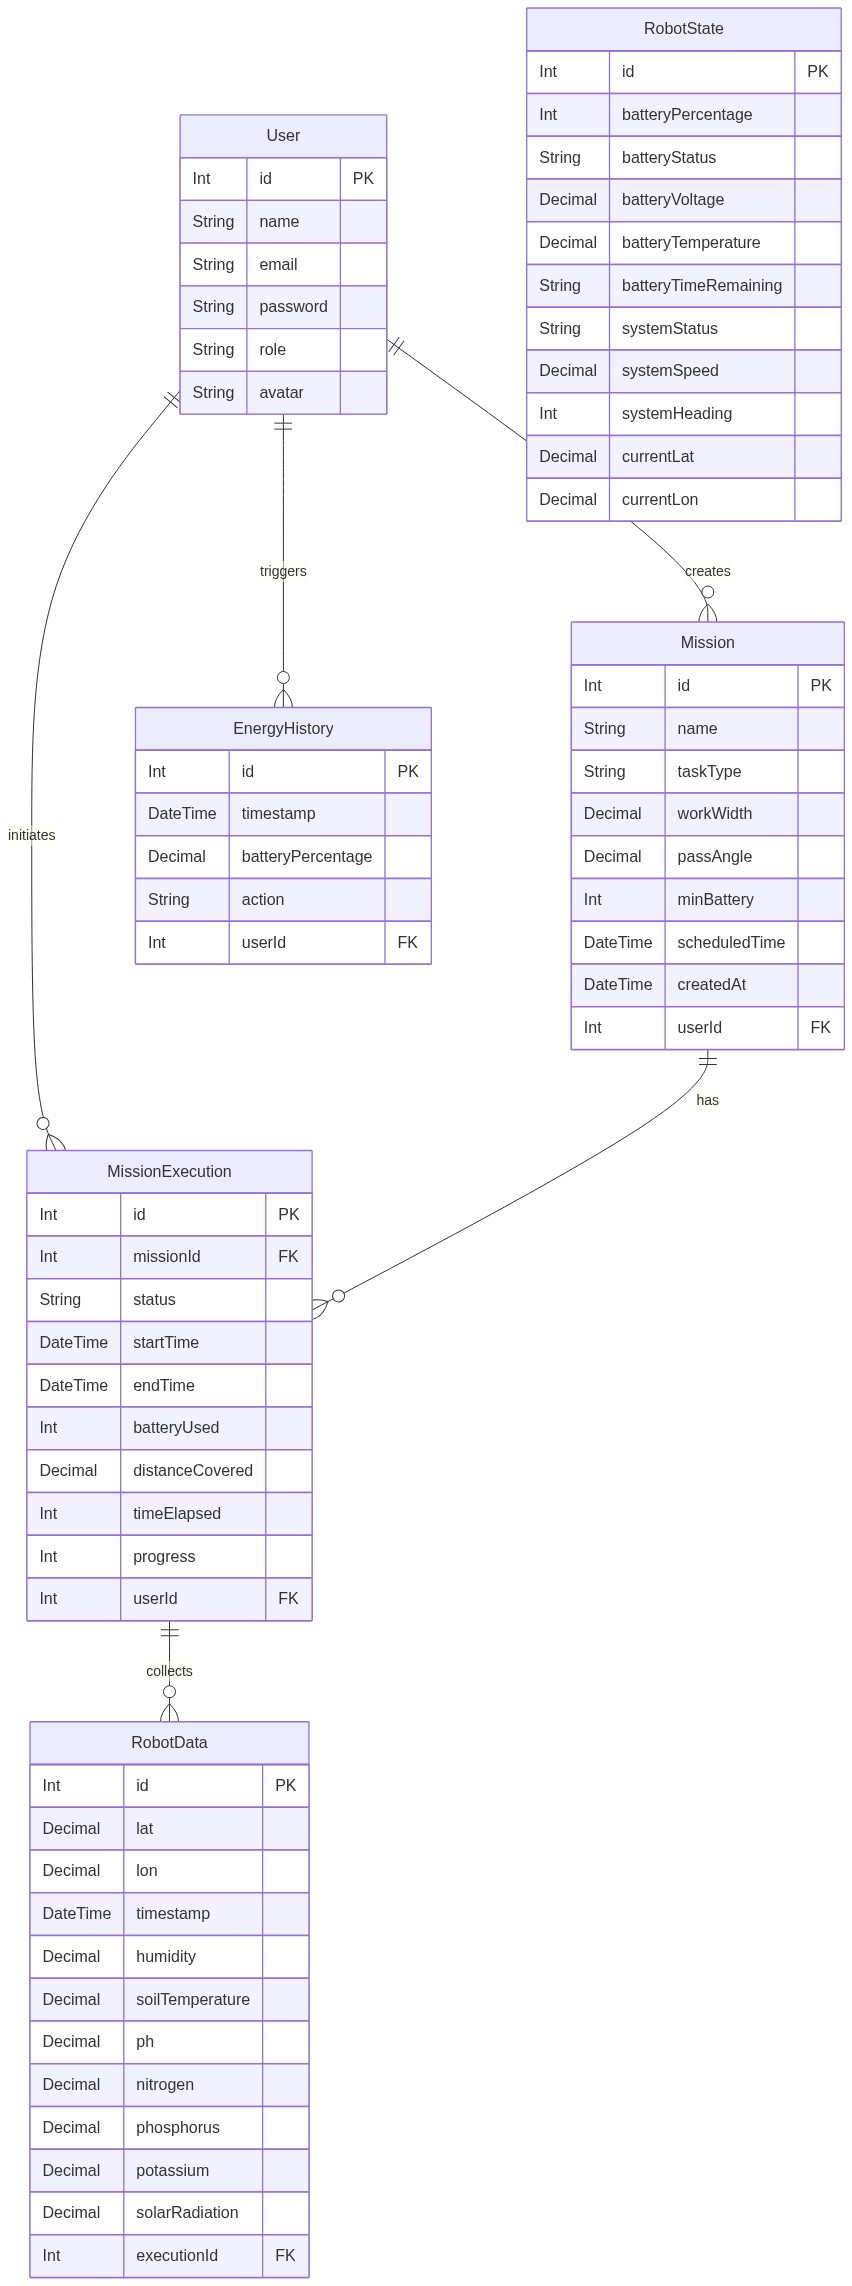
\includegraphics[width=0.95\textwidth,height=0.9\textheight,keepaspectratio]{img/apendice_C/diagrama_bd_final.png}
    \caption{Diagrama Entidad-Relación Lógico del Sistema}\label{fig:img/apendice_C/diagrama_bd_final.png}
\end{figure}

\section{Diseño procedimental}
Este apartado desciende desde la abstracción de los modelos relacionales hacia la sala de máquinas del \textit{software}. Aquí se detallan las especificaciones técnicas, los patrones de diseño arquitectónicos~\cite{designpatterns} adoptados para resolver problemas recurrentes y la lógica algorítmica fundamental (el motor de simulación) que gobierna el comportamiento interno de AgroSkopos.

\subsection{Patrones de diseño utilizados}
El código de la aplicación se ha estructurado siguiendo paradigmas consolidados para garantizar mantenibilidad, alta cohesión y bajo acoplamiento tanto en el \textit{backend} como en el \textit{frontend}.

\subsubsection{Patrones en el servidor (Node.js)}
\begin{itemize}
    \item \textbf{Arquitectura Multicapa (Controller-Service-Repository):} Las peticiones HTTP entrantes son interceptadas por un \textit{Router} que delega en un \textit{Controller}. Este último se apoya en un \textit{Service} que contiene la lógica de negocio pura, aislando las interacciones de base de datos a la capa del repositorio (Prisma). Esta separación previene la existencia de "controladores engordados" (\textit{fat controllers}).
    \item \textbf{Patrón Singleton y Motor de Estado:} El corazón del sistema (el archivo \texttt{simulator.js}) opera bajo un patrón Singleton. Al importarse como módulo de Node.js, mantiene una única instancia en memoria (un cierre léxico o \textit{closure}) que preserva el estado global de la simulación del robot para todos los usuarios concurrentes, sin necesidad de consultar el disco continuamente.
    \item \textbf{Patrón Observer (Pub-Sub):} Implementado a través de WebSockets (\textit{Socket.io}). El servidor actúa como publicador emitiendo métricas (\textit{robot:new\_data}), mientras que los clientes web actúan como suscriptores reactivos, actualizando sus interfaces sin peticiones activas (\textit{polling}).
    \item \textbf{Middlewares y validación de entrada:} Se emplea un patrón de interceptación en las rutas de Express mediante validadores esquemáticos (Zod). Esto asegura que ninguna petición con cuerpo malformado o sin \textit{token} JWT alcance la lógica de dominio.
\end{itemize}

\subsubsection{Patrones en el cliente web (React)}
\begin{itemize}
    \item \textbf{Gestión de Estado Global (Patrón Store con Zustand):} Se ha centralizado la gestión del estado de la aplicación utilizando múltiples \textit{stores} independientes. Esto incluye \texttt{authStore} para la sesión de usuario, \texttt{robotStore} para la telemetría en tiempo real y \texttt{themeStore} para las preferencias visuales, eliminando de raíz la necesidad de la clásica \textit{Context API} y atajando problemas de renderizados innecesarios y el antipatrón de \textit{prop-drilling}.
    \item \textbf{Gestión de Estado del Servidor (TanStack Query):} Para la obtención, almacenamiento en caché y sincronización de datos asíncronos de la API REST (como el histórico de misiones), se emplea \textbf{React Query}. Este patrón reemplaza el uso clásico e imperativo de \texttt{useEffect}, aportando invalidación inteligente de caché y manejo declarativo de estados de carga y error.
\end{itemize}

\subsection{Algoritmia de simulación pesada}
A diferencia de los sistemas de gestión tradicionales orientados a modelos anémicos, el \textit{backend} de AgroSkopos asume el reto de emular un entorno de agricultura de precisión interactivo en tiempo real mediante dos lógicas circulares:

\begin{enumerate}
    \item \textbf{Bucle de Físicas (Energía y Batería):} El servidor realiza un cálculo continuo de recarga solar. La función \texttt{calculateSolarRadiation(date)} modela matemáticamente la posición del sol basándose en la fecha, hora y coordenadas geográficas para devolver un valor en W/m$^2$, que a su vez se traduce en amperaje de recarga. Este proceso combate en paralelo con el consumo paramétrico derivado del estado del motor (IDLE vs WORKING).
    \item \textbf{Bucle Agronómico y Búfer Circular:} Durante el \textit{pathfinding} (\texttt{generateCoveragePath}), el robot emite puntos GPS interpolados. En cada coordenada, un algoritmo pseudoaleatorio criptográficamente seguro inyecta valores de NPK y pH acordes al bioma simulado. Para prevenir la sobrecarga de la base de datos PostgreSQL, la simulación opera como un \textbf{búfer circular}, ejecutando de forma asíncrona sentencias SQL de limpieza (\texttt{DELETE ... NOT IN (SELECT ... LIMIT N)}) que preservan únicamente el histórico reciente, optimizando drásticamente el consumo de RAM.
\end{enumerate}

Para formalizar el comportamiento dinámico del robot durante estas simulaciones, la figura \ref{fig:img/apendice_C/diagrama_estados.png} modela la \textbf{Máquina de Estados Finita} que rige las transiciones del motor interno en respuesta a los comandos y sensores.

\imagen{img/apendice_C/diagrama_estados.png}{Diagrama de Máquina de Estados del Motor de Simulación Agrícola}{0.95}

\subsection{Flujos principales del sistema}
A continuación, se ilustran a través de diagramas de secuencia UML los cinco flujos operacionales más críticos de la arquitectura.

\subsubsection{Flujo de Autenticación y Autorización}
El primer punto de contacto de cualquier operario con el sistema es el inicio de sesión (figura \ref{fig:img/apendice_C/flujo_autenticacion.png}). Los pasos son los siguientes:
\begin{enumerate}
    \item El usuario introduce sus credenciales en el formulario de la aplicación web y el \textit{frontend} envía la petición POST al \textit{backend}.
    \item El \textit{backend} (Express) busca al usuario en la base de datos a través del ORM Prisma.
    \item Se verifica la validez de la contraseña comparándola con el \textit{hash} almacenado utilizando la librería \texttt{bcrypt}.
    \item Si las credenciales son válidas, el sistema genera y firma un \textit{JSON Web Token} (JWT) que se devuelve al cliente.
    \item El \textit{Context API} de React almacena el \textit{token} en memoria local, utilizándolo a partir de ese momento para autorizar de forma segura las futuras peticiones al API.
\end{enumerate}

\imagen{img/apendice_C/flujo_autenticacion.png}{Diagrama de Secuencia: Flujo de Autenticación}{0.95}

\subsubsection{Flujo de Planificación de Misión Agrícola}
Antes de ejecutar una tarea, el sistema requiere una planificación espacial (figura \ref{fig:img/apendice_C/flujo_planificacion.png}). El proceso de creación es el siguiente:
\begin{enumerate}
    \item El operario utiliza la capa interactiva del mapa en React para trazar visualmente un polígono cerrado sobre la parcela.
    \item El \textit{frontend} recolecta estos puntos geográficos, calcula el área teórica y los formatea al estándar \textit{GeoJSON}.
    \item El usuario completa el resto del formulario (nombre, tipo de cultivo, tarea) y lo envía al servidor.
    \item El API intercepta el paquete y un \textit{middleware} valida la estandarización geométrica de las coordenadas utilizando Zod.
    \item Si la validación es exitosa, se persiste la nueva misión en la base de datos y se redirige al usuario a la lista de tareas pendientes.
\end{enumerate}

\imagen{img/apendice_C/flujo_planificacion.png}{Diagrama de Secuencia: Planificación de Cobertura Agrícola}{0.95}

\subsubsection{Flujo de Ejecución de Misión}
La transición de una misión desde su fase de planificación estática hasta su ejecución dinámica en el terreno se detalla en la figura \ref{fig:img/apendice_C/flujo_mision.png}:
\begin{enumerate}
    \item El operario localiza una misión en estado pendiente y pulsa el botón de \textit{Iniciar} desde el panel de control.
    \item El \textit{backend} recibe la instrucción y comprueba las precondiciones operativas, asegurando que el robot cuente con la batería mínima requerida.
    \item Se genera un nuevo registro en la tabla \texttt{ejecuciones\_mision} para trazar el marco temporal de la tarea.
    \item El servidor activa el contexto en la memoria del simulador y el motor matemático calcula la ruta de cobertura de área (\textit{pathfinding}).
    \item Se notifica instantáneamente a todos los clientes a través del bus de eventos (Socket.io). El gestor de estado (\textit{Zustand}) actualiza la interfaz en vivo mostrando al robot desplazándose.
\end{enumerate}

\imagen{img/apendice_C/flujo_mision.png}{Diagrama de Secuencia: Inicio de una Misión Agrícola}{0.95}

\subsubsection{Ciclo de Vida de Telemetría (Real-Time)}
El flujo más recurrente y pesado del proyecto es la captación continua de telemetría (figura \ref{fig:img/apendice_C/flujo_telemetria.png}), que actúa como el "latido" del sistema:
\begin{enumerate}
    \item El intervalo asíncrono interno de Node.js se dispara periódicamente, actuando como el reloj maestro de la simulación.
    \item El motor de físicas recalcula la recarga de los paneles solares y el drenaje de la batería basándose en el clima y el estado actual.
    \item El motor agronómico interpola la nueva posición GPS en el terreno y simula lecturas de NPK y pH inyectando valores semi-aleatorios atados a una semilla criptográfica.
    \item Los datos resultantes se persisten de forma masiva en PostgreSQL, activando en paralelo el algoritmo de limpieza de búfer circular.
    \item Finalmente, el servidor emite el paquete JSON comprimido por WebSockets. React recibe los paquetes y fuerza el redibujado instantáneo de la posición y mapas de calor.
\end{enumerate}

\imagen{img/apendice_C/flujo_telemetria.png}{Diagrama de Secuencia: Ciclo de Telemetría Asíncrona}{0.95}

Para comprender mejor cómo se establece y mantiene este canal de comunicación bidireccional en tiempo real entre los múltiples clientes y el servidor sin bloqueos, la figura \ref{fig:img/apendice_C/arquitectura_websockets.png} ilustra la arquitectura lógica de la conexión por WebSockets:

\imagen{img/apendice_C/arquitectura_websockets.png}{Diagrama de Arquitectura de red: Conexiones mediante WebSockets}{0.95}

\subsubsection{Consulta de Histórico y Análisis Energético}
Para permitir la toma de decisiones, la aplicación consolida el rendimiento pasado del robot en gráficas interactivas (figura \ref{fig:img/apendice_C/flujo_analitica.png}):
\begin{enumerate}
    \item El administrador accede a la sección de analíticas desde la barra de navegación lateral.
    \item React despacha peticiones HTTP REST concurrentes al \textit{backend} solicitando datos agregados.
    \item Prisma ejecuta sentencias complejas de extracción en la tabla de \texttt{robot\_datos} y en \texttt{historial\_energia}.
    \item El servidor Node.js unifica, pagina y filtra las matrices de resultados, devolviéndolas serializadas.
    \item El componente de \textit{frontend} formatea la estructura de los datos para inyectarlos en la librería visual Recharts, renderizando finalmente las curvas de rendimiento.
\end{enumerate}

\imagen{img/apendice_C/flujo_analitica.png}{Diagrama de Secuencia: Flujo de Visualización Analítica}{0.95}

\subsubsection{Flujo de Registro de Usuario y Notificación Asíncrona}
El proceso de alta de nuevos empleados combina operaciones síncronas de base de datos con delegación asíncrona de correos (figura \ref{fig:img/apendice_C/flujo_notificacion.png}):
\begin{enumerate}
    \item El administrador rellena el formulario de alta y el \textit{frontend} envía la petición POST al servidor.
    \item El servidor valida la autorización (que el usuario origen posea rol de administrador) y comprueba el formato con Zod.
    \item Prisma inserta el nuevo usuario en la base de datos PostgreSQL, autogenerando una contraseña temporal en texto plano o enlazando el correo.
    \item El sistema no bloquea el hilo para enviar el correo: en su lugar, encola el trabajo \texttt{send-welcome-email} en el bróker de Redis gestionado por BullMQ.
    \item El servidor responde inmediatamente al administrador con un estado HTTP 201 (Creado), liberando la interfaz del cliente web.
    \item En segundo plano, un trabajador (\textit{Worker}) extrae la tarea de Redis, compila la plantilla HTML, y la transmite mediante Nodemailer al servidor \textbf{SMTP}, notificando finalmente al usuario recién dado de alta.
\end{enumerate}

\imagen{img/apendice_C/flujo_notificacion.png}{Diagrama de Secuencia: Alta de usuario y colas asíncronas}{0.95}

\subsubsection{Flujo de Soporte Técnico por Tickets}
De manera análoga al envío de credenciales, el sistema protege el rendimiento frente a posibles latencias de red durante el reporte de incidencias técnicas (figura \ref{fig:img/apendice_C/flujo_tickets.png}):
\begin{enumerate}
    \item El usuario detecta un error y envía un reporte desde la sección de soporte.
    \item El \textit{backend} valida la petición y la vincula de forma segura con el operario solicitante, extrayendo la identidad directamente del \textit{token} JWT en lugar del cuerpo de la petición.
    \item El sistema encola un trabajo de tipo \texttt{send-ticket-email} en Redis.
    \item La interfaz web muestra una confirmación instantánea al usuario de que la incidencia ha sido registrada correctamente.
    \item Posteriormente, el servicio en segundo plano formatea los datos y transmite un correo electrónico detallado al departamento técnico.
\end{enumerate}

\imagen{img/apendice_C/flujo_tickets.png}{Diagrama de Secuencia: Reporte de incidencias y Sistema de Tickets}{0.95}

\section{Diseño arquitectónico}
En esta sección se define la estructura global del sistema, la organización de sus repositorios lógicos y las reglas que rigen la comunicación entre ellos. Para AgroSkopos, se ha optado por una arquitectura de alto rendimiento orientada a eventos y procesamiento geoespacial, desmarcándose fuertemente de los sistemas de gestión tradicionales.

\subsection{Arquitectura Global e Infraestructura}
El sistema implementa un modelo de arquitectura cliente-servidor completamente desacoplado y regido por un \textbf{Protocolo Dual}. A diferencia de las aplicaciones web convencionales basadas estrictamente en transferencias de estado (REST), donde el cliente debe sondear continuamente al servidor en busca de cambios (\textit{polling}), AgroSkopos utiliza un enfoque híbrido para optimizar la carga de red:
\begin{itemize}
    \item \textbf{Canal transaccional (HTTP/REST):} Empleado para operaciones de ciclo de vida largo, estáticas y que requieren validación rigurosa, como la autenticación de operarios, la consulta de históricos o la inserción de nuevas misiones en la base de datos.
    \item \textbf{Canal de flujo continuo (WebSockets):} Empleado para mantener una conexión TCP persistente, bidireccional y \textit{stateful} entre el servidor y los clientes. Este patrón (\textit{Pub-Sub}) permite que el motor de simulación emita un \textit{stream} ininterrumpido de telemetría a alta frecuencia, garantizando que el mapa interactivo se mueva en tiempo real con una latencia mínima.
\end{itemize}

Para facilitar la comprensión visual de estas interacciones, se han elaborado dos esquemas. La figura \ref{fig:img/apendice_C/arquitectura_cliente_servidor.png} detalla las tecnologías lógicas empleadas en cada capa de la aplicación. Por otro lado, la figura \ref{fig:img/apendice_C/arquitectura_docker.png} ilustra la arquitectura de despliegue físico.

% DIAGRAMAS (El usuario exportará los PNG desde Draw.io)
\imagen{img/apendice_C/arquitectura_cliente_servidor.png}{Diagrama de Arquitectura de Software: Interacción entre Cliente, Servidor y Base de Datos}{0.95}

A nivel de infraestructura, el sistema se apoya íntegramente en la contenerización mediante \textbf{Docker}. Al orquestar los servicios con \texttt{docker-compose}, se levantan cuatro contenedores lógicos aislados: la base de datos relacional (PostgreSQL), el motor en memoria (Redis), el motor API (Node.js) y el servidor de estáticos del \textit{frontend} (Nginx~\cite{nginx}). Esta separación garantiza que los entornos de desarrollo, pruebas y producción sean idénticos, evitando el clásico problema de "funciona en mi máquina".

\imagen{img/apendice_C/arquitectura_docker.png}{Diagrama de Infraestructura y Despliegue: Contenedores Docker}{0.95}

\subsection{Arquitectura del Backend (Node.js)}
El servidor central de AgroSkopos está desarrollado sobre el entorno de ejecución asíncrono Node.js utilizando el \textit{framework} Express. La decisión de usar Node.js radica en su arquitectura no bloqueante (basada en el \textit{Event Loop}), la cual es excepcionalmente brillante para manejar miles de conexiones simultáneas por WebSockets sin agotar los hilos del procesador.

El \textit{backend} abandona el concepto pasivo habitual para convertirse en un \textbf{Motor Activo}. Normalmente, un servidor web permanece inactivo hasta que recibe una petición HTTP. Sin embargo, este servidor ejecuta un bucle de simulación interno (\texttt{simulator.js}) que corre de fondo ininterrumpidamente, calculando variables agronómicas, consumo de batería y geolocalización, independientemente de si hay clientes conectados o no.

Las tecnologías clave que sostienen la arquitectura del servidor (cuyas interacciones internas se detallan visualmente en la figura \ref{fig:img/apendice_C/arquitectura_backend.png}) son:
\begin{itemize}
    \item \textbf{Enrutamiento y Control (Express):} Gestiona el ciclo de vida de las peticiones HTTP y aplica las políticas de control de acceso cruzado (\textbf{CORS}).
    \item \textbf{Capa de Validación Rigurosa (Zod):} Se adopta una política de \textit{fail-fast}. Antes de que cualquier paquete de datos alcance los controladores, los \textit{middlewares} interceptan el \textit{payload} y lo comparan contra esquemas matemáticos estrictos utilizando la librería Zod. Esto previene eficazmente inyecciones \textbf{NoSQL} y asegura que las coordenadas geográficas mantengan su integridad.
    \item \textbf{Análisis Espacial (Turf.js):} Dado que la aplicación es altamente geográfica, el servidor incorpora \texttt{@turf/turf} para realizar proyecciones geométricas y calcular áreas de polígonos interceptados sin necesidad de delegar este cálculo a PostGIS, reduciendo la carga transaccional de la base de datos.
    \item \textbf{Capa de Persistencia (Prisma ORM):} En contraposición a escribir sentencias \textbf{SQL} en crudo, se utiliza Prisma como Mapeador Objeto-Relacional. Prisma garantiza seguridad de tipos (\textit{Type-Safety}) durante las operaciones \textbf{CRUD}, evitando errores humanos durante el desarrollo e inyecciones SQL en tiempo de ejecución.
    \item \textbf{Auto-Documentación Estándar (Swagger/OpenAPI):} La interfaz del API REST no es opaca. Se han integrado las librerías \texttt{swagger-jsdoc} y \texttt{swagger-ui-express} para generar en tiempo real una interfaz interactiva de documentación técnica. Esto permite auditar los \textit{endpoints}, \textit{payloads} y códigos de estado HTTP directamente desde el navegador, cumpliendo con los estándares de diseño \textit{API-First}.
\end{itemize}

\imagen{img/apendice_C/arquitectura_backend.png}{Diagrama de Arquitectura Interna del \textit{Backend} (Node.js y Motor Activo)}{0.95}

\subsection{Arquitectura del \textit{Frontend} (React)}
El cliente web está diseñado bajo el paradigma de las \textit{Single-Page Applications} (\textbf{SPA})~\cite{spa}. En lugar de renderizar el HTML en el servidor para cada clic, la interfaz se carga una sola vez en el navegador y muta de forma dinámica, ofreciendo una experiencia fluida equivalente a la de un \textit{software} de escritorio nativo. 

Para lograr tiempos de compilación instantáneos, se ha prescindido de los empaquetadores heredados como \textit{Webpack} en favor de \textbf{Vite}. Acoplado con el compilador SWC (escrito en Rust), la aplicación se levanta en milisegundos durante el desarrollo.

La arquitectura del cliente se subdivide en las siguientes áreas tecnológicas de alta complejidad:
\begin{itemize}
    \item \textbf{Subsistema de Información Geográfica (Capa GIS):} Constituye el núcleo central visual de la plataforma. El lienzo del mapa está motorizado por \texttt{leaflet} e integrado en el ciclo de vida de los componentes mediante \texttt{react-leaflet}. La trazabilidad interactiva (cuando el operario dibuja el área de trabajo) recae sobre la librería \texttt{@geoman-io/leaflet-geoman-free}. Además, las capas topológicas que representan las lecturas agronómicas del simulador son interpoladas visualmente mediante \texttt{leaflet.heat}.
    \item \textbf{Gestor de Estado Global (Zustand):} Uno de los mayores retos arquitectónicos de una SPA compleja es evitar el \textit{prop-drilling} (pasar datos entre docenas de componentes anidados). En lugar de emplear Redux, que añade una verbosidad excesiva y ralentiza el desarrollo, se ha integrado \textbf{Zustand}. Este almacén inyecta la telemetría recibida por WebSockets directamente a los marcadores del mapa y a las gráficas, aislando los renderizados innecesarios.
    \item \textbf{Diseño Responsivo y PWA (\textit{Progressive Web App}):} La interfaz ha sido maquetada utilizando \textbf{CSS modular} y \textit{Media Queries} fluidas, garantizando que el cuadro de mandos sea perfectamente operable tanto en monitores de centro de control como en las \textit{tablets} rugerizadas de los operarios a pie de campo. Adicionalmente, el proyecto integra el conector \texttt{vite-plugin-pwa}, permitiendo que la web se instale como una aplicación nativa en dispositivos móviles y cachee sus recursos estáticos (\textit{Service Workers}), una característica vital para operar en parcelas agrícolas con conectividad intermitente.
    \item \textbf{Analítica de Datos (Recharts):} La visualización de históricos de carga energética y avance de misión se delega en la librería vectorial \texttt{recharts}, que procesa matrices masivas de datos para dibujar gráficos de líneas interactivos en \textbf{SVG}.
    \item \textbf{Exportación Documental e Internacionalización:} Dado que la plataforma puede operar en diversos entornos, incorpora \texttt{i18next} para abstraer las cadenas de texto y permitir el cambio de idioma en caliente sin recargar. Adicionalmente, el ecosistema integra \texttt{html2canvas} junto con \texttt{jsPDF} para vectorizar las gráficas de rendimiento y ofrecer a los responsables la capacidad de exportar informes físicos en formato \textbf{PDF} con un solo clic.
\end{itemize}

\subsection{Modelo de Seguridad, Resiliencia y Mitigación de Ataques}
Dado que el \textit{software} emula un entorno agro-industrial crítico, la arquitectura ha sido reforzada a nivel \textit{DevOps} incorporando mitigadores directos frente a ataques cibernéticos modernos y fallos en tiempo de ejecución:

\imagen{img/apendice_C/modelo_seguridad.png}{Diagrama de Arquitectura: Topología y Capas de Seguridad Perimetral}{0.95}

\begin{enumerate}
    \item \textbf{Identidad y Control de Acceso (RBAC):} El control de autorización se implementa mediante el modelo \textit{Role-Based Access Control~\cite{rbac}} (Administrador, Operario, Visualizador). El estado de autenticación no se guarda en memoria del servidor (\textit{stateless}), sino que fluye encapsulado y firmado criptográficamente en \textit{JSON Web Tokens} (\textbf{JWT}). Para prevenir robos de sesión, el token no es accesible por JavaScript, sino que se transfiere mediante una \textit{cookie} \texttt{httpOnly} gestionada con \texttt{cookie-parser}. Las contraseñas están ofuscadas en base de datos mediante el algoritmo de coste adaptativo \texttt{bcrypt}.
    \item \textbf{Prevención de DDoS (Denegación de Servicio):} Las infraestructuras conectadas a la red corren el riesgo de ser saturadas por peticiones masivas. Se ha integrado la librería \texttt{express-rate-limit} a nivel de enrutador raíz, la cual estrangula proactivamente el tráfico si una misma IP excede el umbral seguro de 200 peticiones en 15 minutos.
    \item \textbf{Prevención de Memory Exhaustion:} La ingestión de polígonos y datos geoespaciales es un vector de ataque clásico para desbordar la memoria RAM. El sistema está acorazado explícitamente mediante el interceptor \texttt{express.json(\{ limit: "1mb" \})}, descartando instantáneamente cargas maliciosas o excesivamente pesadas antes de que sean procesadas por la lógica de dominio.
    \item \textbf{Cabeceras Seguras y Geofencing Lógico:} El módulo \texttt{helmet} reescribe activamente las respuestas HTTP para prevenir ataques \textbf{XSS} (\textit{Cross-Site Scripting}) mediante la inyección de \textit{Content-Security-Policies} (\textbf{CSP}). Adicionalmente, dado que un robot agrícola suele operar en redes LAN aisladas, el cortafuegos lógico \textbf{CORS} rechaza taxativamente el tráfico que no proceda del \textit{localhost} o de subredes autorizadas (ej. \texttt{192.168.x.x}).
    \item \textbf{Proxy Inverso para Evitar Bloqueos HTTPS:} Para garantizar el envío y validación de la \textit{cookie} \texttt{httpOnly} bajo entornos estrictos en \textbf{HTTPS} (y en modo incógnito en Chrome/Edge), el \textit{frontend} en Vercel actúa como \textit{proxy} inverso nativo (\texttt{vercel.json}). Esto sortea las restricciones \textit{Cross-Site} haciendo que el navegador interprete que tanto el \textit{frontend} como el \textit{backend} (Azure) operan exactamente en el mismo dominio de origen (\textit{First-Party}).
    \item \textbf{Resiliencia de Subprocesos (\textit{Crash Prevention}):} Node.js tiene un comportamiento determinista de colapso frente a promesas huérfanas. Para evitar que una anomalía matemática del simulador apague el servidor entero, el archivo principal implementa escuchadores activos (\texttt{uncaughtException} y \texttt{unhandledRejection}) que atrapan la excepción en memoria, imprimen una traza en el log y degradan el servicio de manera elegante sin corromper el estado de la máquina física real.
\end{enumerate}

\subsection{Arquitectura de Pruebas y Control de Calidad (QA)}
Para asegurar la robustez de un sistema con lógicas tan pesadas como el \textit{pathfinding} geográfico y la simulación matemática, se ha implantado una infraestructura de pruebas de grado industrial.

En lugar de basar la fiabilidad en la simple comprobación manual del desarrollador, el proyecto incluye \textit{suites} de pruebas automatizadas:
\begin{itemize}
    \item \textbf{Frontend (Vitest):} Se utiliza Vitest, el \textit{framework} de pruebas nativo de Vite, para aislar y validar el comportamiento de los componentes React y funciones puras de utilidad de manera ultrarrápida en entornos de terminal.
    \item \textbf{Backend (Jest y Supertest):} La lógica de servidor cuenta con pruebas asiladas gobernadas por Jest. La librería \texttt{supertest} actúa como un agente HTTP falso que bombardea el API REST y valida los códigos de estado devueltos (200 OK, 403 Forbidden, 400 Bad Request) y la estandarización JSON de las respuestas.
    \item \textbf{Pruebas End-to-End (Testcontainers):} Probablemente la tecnología más avanzada de la fase \textbf{QA}. En los \textit{tests} de integración profundos (\textit{E2E}), el sistema utiliza \texttt{@testcontainers/postgresql}. Esto significa que, durante la ejecución del \textit{test}, Node.js se comunica con el demonio de Docker del ordenador para levantar dinámicamente un contenedor efímero real de PostgreSQL, inyectar datos de prueba, realizar las afirmaciones (\textit{assertions}) pertinentes, y destruir el contenedor al finalizar. De este modo, se verifica la interacción real entre el ORM Prisma y el motor relacional sin riesgo de contaminar la base de datos de producción.
    \item \textbf{Pruebas de Carga y Rendimiento (k6):} Para simular situaciones de alto estrés (como múltiples agricultores operando misiones y robots emitiendo telemetría ininterrumpida simultáneamente), se han implementado \textit{scripts} de \textbf{k6} orientados a pruebas de humo (\textit{Smoke}), estrés (\textit{Stress}), picos (\textit{Spike}) y remojo (\textit{Soak}). Esto permite analizar el comportamiento asíncrono y los límites de rotura del sistema antes del despliegue.
    \item \textbf{Integración y Despliegue Continuo (CI/CD):} Toda esta batería de calidad, incluyendo el escáner de deuda técnica y métricas de código (SonarCloud), no se ejecuta manualmente. Está totalmente automatizada mediante \textbf{GitHub Actions}. Cada \textit{commit} de código empujado a la rama de desarrollo dispara servidores virtuales automáticos que evalúan rigurosamente todo el ecosistema de \textit{software}, bloqueando errores que comprometan la aplicación.
\end{itemize}
